%  !TeX  root  =  user_guide.tex

\section{Offline Editing Plugin}\label{sec:offlinedit}

% when the revision of a section has been finalized, 
% comment out the following line:
\updatedisclaimer

For data collection, it is a common situation to work with a laptop or a cell 
phone offline in the field. Upon returning to the network, the changes need to 
be synchronized with the master data source, e.g. a PostGIS database. If several 
persons are working simultaneously on the same datasets, it is difficult to 
merge the edits by hand, even if people don't change the same features.

The \toolbtntwo{offline_editing_copy}{Offline Editing} Plugin automates the 
synchronisation by copying the content of a datasource (usually PostGIS or 
WFS-T) to a spatialite database and storing the offline edits to dedicated 
tables. After being connected to the network again, it is possible to apply 
the offline edits to the master dataset.

\minisec{Using the plugin}

\begin{itemize}
\item Open some vector layers, e.g. from a PostGIS or WFS-T datasource
\item Save it as a project
\item Press the 'Convert to offline project' button and select the layers to 
save. The content of the layers is saved to spatialite tables.
\item Edit the layers offline.
\item After being connected again, upload the changes with the 'Synchronize' 
button.
\end{itemize}

\begin{figure}[ht]
   \centering
   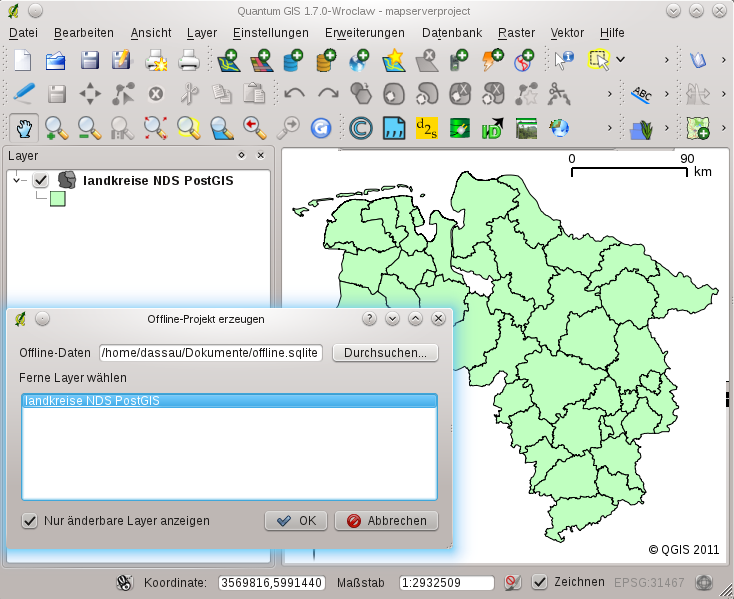
\includegraphics[clip=true, width=12cm]{create_offline_project}   
   \caption{Create an offline project from PostGIS or WFS layers \nixcaption}
   \label{fig:offlineproject}
\end{figure}

\FloatBarrier
